\begin{document}
   
We can divide our experiments across two categories, facial expression recognition, keyboard dynamics, and mouse dynamics.
We will also discuss our data gathering techniques here. Data gathering based on mood induction was performed in a controlled environment. 
First, each participant was exposed to a series of videos that are emotion-inducing. 
Every video is meant to induce a specific emotion, such as a happy video to induce happiness, a sad video to induce sadness, Etc, 
in order to try to collect a wider variety of emotions.
Some of the videos were taken by the suggestion of Rumpa et el. \cite{exp_videos} and some from social media.

\begin{figure}[htp]
    \centering
    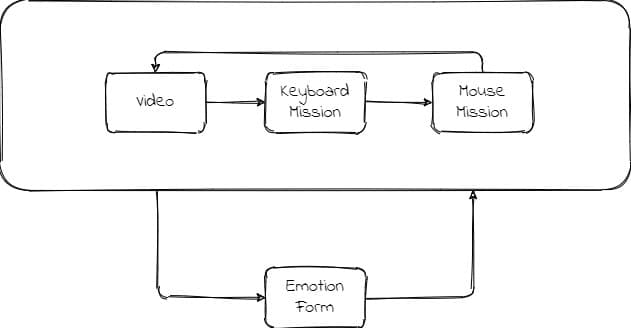
\includegraphics[width=10cm]{figures/exp_flow}   
    \caption{State machine diagram describing the flow of the expirement.}
    \label{fig:exp_flow} 
\end{figure}

\begin{figure}[htp]
    \centering
    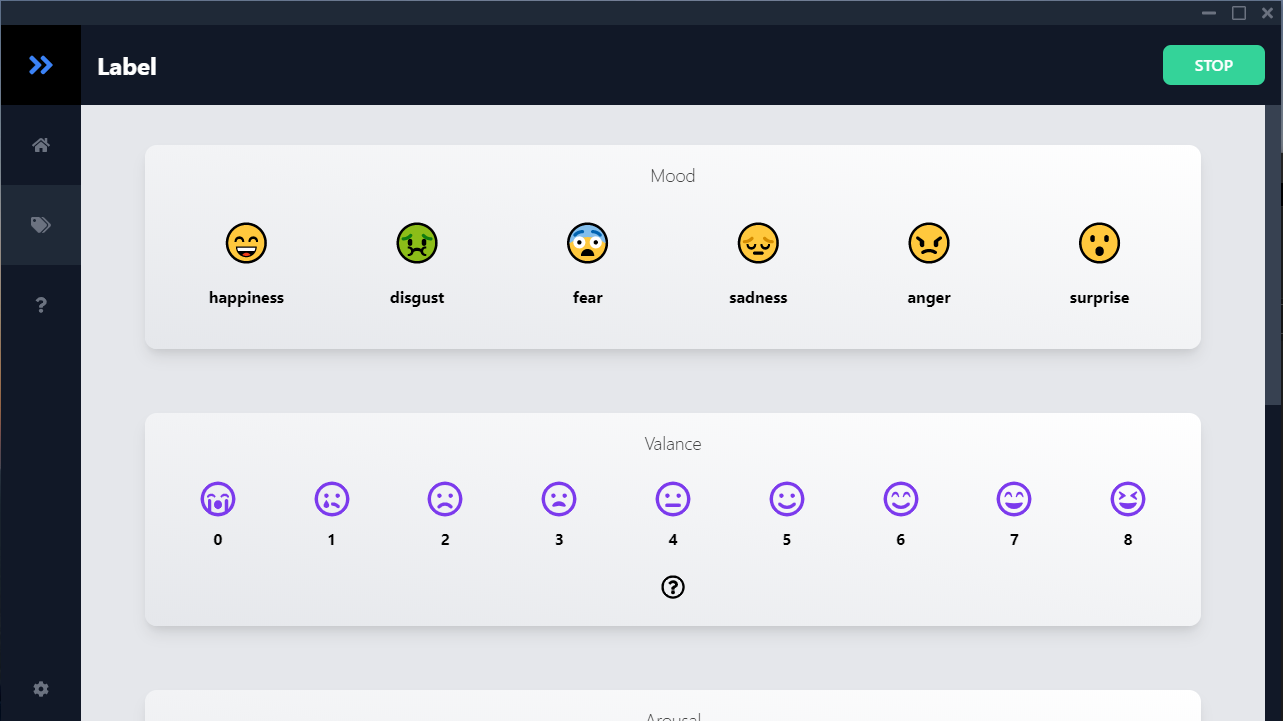
\includegraphics[width=10cm]{figures/collection_ui}   
    \caption{Collection system user interface.}
    \label{fig:collection_ui} 
\end{figure}

Second, after every video, the participant had to complete a mission using the keyboard and another mission using the mouse. 
On the keyboard-based task, after every video, the participant had to write what he saw (in Hebrew) and write the first stanza from the poem 
"The Road not Taken" (in English). On the mouse-based task, after every video, the participant had to play a game 
called Bubble Shooter for around 2-4 minutes. In the game, the participant needs to move the mouse over different angles and 
shoot balls in different colors by clicking on the mouse to match series of balls in the same color. Every minute, 
the participant had to answer a form in which he was asked how he felt in different perspectives. 



We recorded the participants on the different channels during the whole experiment and labeled their emotions on the VAD scale \cite{VAD_model} 
and the corresponding categorical emotions scale based on Ekman's emotions \cite{Ekman_Theory}. 
Every single experiment took around 30 to 60 minutes. \ref{fig:exp_flow}
In order to record and save the data from the user, 
we used our application. While the application was recording, it collected all the inputs from the different channels - recorded events from the keyboard 
and the mouse and took pictures of the participant with two frames per second. Every minute, 
the application asked the user for his emotions, and the user could easily fill the form and continue the experiment \ref{fig:collection_ui}. 
Further information about our application for data gathering is available in the appendix \ref{appendix:collection_system}

\end{document}
